\label{cap:implementierung}
F{\"u}r die Umsetzung der im Kapitel \ref{cap:konzept} angesprochenen Ideen und
Eigenschaften wurde die Programmiersprache C++ verwendet. Als
Entwicklungsumgebung kam Eclipse zum Einsatz. Zur Verbesserung der Teamarbeit
und des Austausches von Quellcode wurde ein Github Repository
\footnote{www.github.com} angelegt, welches {\"u}ber das Eclipse-Plugin EGit genutzt wurde. \newline Im Folgenden wird
im Detail auf die Art und Weise der Realisierung der beiden Top-Level-Module
\Code{Sender} und \Code{Receiver} eingegangen. Hierf{\"u}r wurde eine flexible und
modulare Softwarearchitektur entwickelt, damit auf sp{\"a}tere {\"A}nderungen, neue Anforderungen
und erforderliche Optimierungen flexibel reagiert werden kann. Dies ist durch
das einfache Austauschen kompletter Module m{\"o}glich.
Daf{\"u}r wird ein objektorientiertes Design genutzt, womit Quellcoderedundanzen und damit
zahlreiche potentielle Programmierfehler vermieden werden konnten.
Weiterhin ist die Wiederverwendung einzelner Quellcodepassagen m{\"o}glich.\newline
Damit die beiden Module in anderen Projekten einfach genutzt werden k{\"o}nnen,
wurde eine statische Bibliothek erstellt, welche {\"u}ber eine Schnittstelle die
Funktionen der beiden Module bereitstellt. In dieser Arbeit wurden nur die beiden
Datentypen Text und Sensorwerte integriert.

\section{Modulaufbau Sender}

Die Aufgabe des Moduls \Code{Sender} besteht darin, die aus vier Phasen
bestehende Verarbeitung der Daten aus \todo{REF }
%zu 1 CRODT framework final_v1.3 pdf - der mag das iwi nicht im todo
umzusetzen.
In \abbildung{BlockdiagrammSender} ist das Blockdiagramm des Moduls \Code{Sender}
darstellt.
Dies bietet eine {\"U}bersicht zu den Modulen und zeigt wie diese untereinander 
Kommunizieren. In der Grafik ist jedes Submodul durch ein M in der linken
oberen Ecke des Blockes gekennezeichnt. Ebenso ist die Schnittstellenklasse angegeben
und durch die Abk{\"u}rzung IF (Interface) gekennzeichnet. Dadurch ist der geforderte modulare
Aufbau sichergestellt.

\begin{figure}[H]
\centering
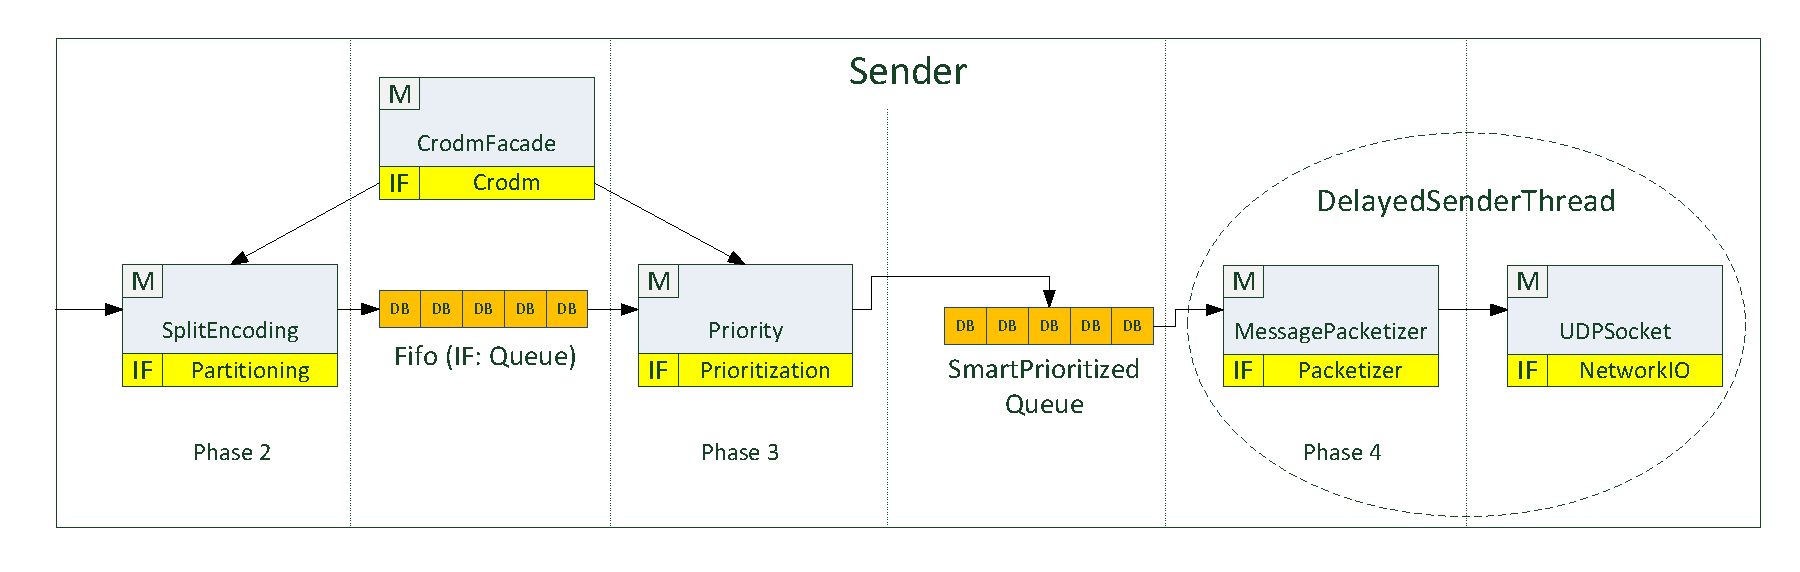
\includegraphics[scale=.5]{BlockdiagrammSender.pdf} % skalieren
\caption{Blockdiagramm des Senders}
\label{fig:BlockdiagrammSender}
\end{figure}

Die Daten werden {\"u}ber die Schnittstelle des Topmoduls {\"u}bergeben und an die
Klasse \Code{Partitionierung} weitergegeben. Dort werden diese, abh{\"a}ngig
ihrer Relevanz, in Datenbl{\"o}cke zerlegt. Zus{\"a}tzlich werden in diesem
Schritt die Datenblockheader (siehe Kapitel \ref{sec:ProtokolDesign}) erstellt und der
Content in bin{\"a}re Daten umgewandelt. Am Ende werden die Datenbl{\"o}cke mit den
Headerinformationen in einer FIFO gepuffert.
Anschliessend wird jedem einzelnen Datenblock im n{\"a}chsten Modul eine Priorit{\"a}t zugewiesen. Die angesprochene
Relevanz und die Priorit{\"a}t der Datenbl{\"o}cke werden in einem extra Modul
namens CRODM (Content Relevance-oriented Data Management)
berechnet und den Modulen {\"u}bergeben.
Anhand dieser wird der Datenblock in die Datenstruktur
\Code{SmartPrioritizedQueue} einsortiert. Dadurch wird
gew{\"a}hrleistet, dass die wichtigen Daten zuerst gesendet werden. F{\"u}r diese
Aufgabe wird eine einfache Liste aus der Standard Template Library (STL)
verwendet. Durch diese kann iteriert werden und es besteht ein schneller
zufälliger Zugriff auf das Element, welches ebenso effektiv eingefügt und
gelöscht werden kann. Weiterhin exsistiert die notwendige Sortierfunktion. Diese
hat f{\"u}r den durch sie ausgef{\"u}hrten Zweck eine vergleichsweise gute
Laufzeit.
Damit die Verz{\"o}gerung, die durch gro{\ss}e Entfernungen auftritt, besser
ber{\"u}cksichtigt werden kann, wird das Submodul \Code{Packetizer} als Thread
gestartet.
Dieser holt sich die Pakete mit der h{\"o}chsten Priorit{\"a}t aus der
\Code{SmartPriorisierendenQueue} und verpackt diese in eine Nachricht, welche
anschlie{\ss}end an die Netzwerkschnittstelle {\"u}bergeben und versandt wird.
\newline Die Umsetzung der Submodule wird im Nachfolgenden genauer
erl{\"a}utert.

\subsection{Splitten und Encoden}

Die Aufgabe des Submoduls \Code{SplitEncoding} ist, die einkommenden Daten
anhand ihrer Relevanz in kleine Datenbl{\"o}cke zu unterteilen. F{\"u}r die Entwicklung
des daf{\"u}r erforderlichen Algorithmus wurde der in \abbildung{Beispieltext}
dargestellte Beispieltext erstellt.

\begin{figure}[H]
\centering
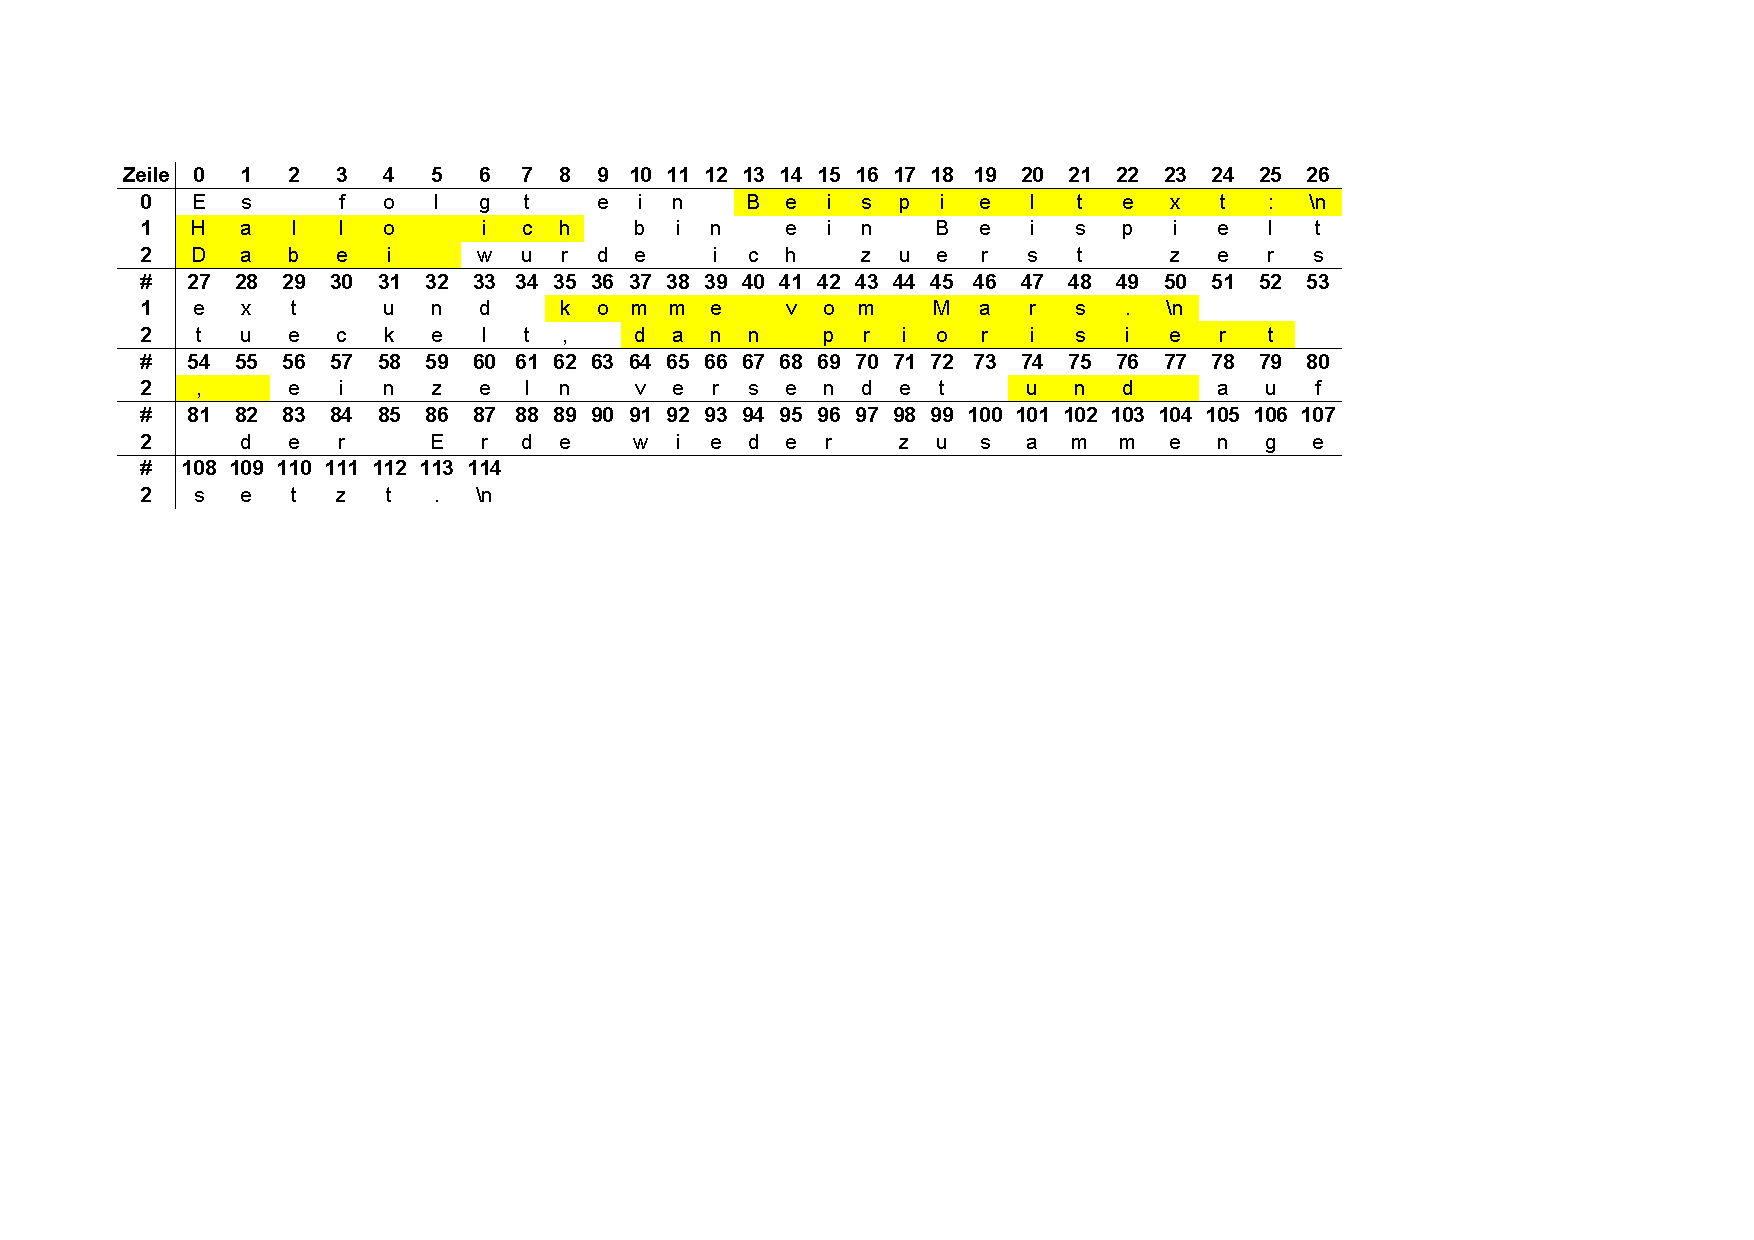
\includegraphics[scale=.4]{Beispieltext.pdf}
\caption{Beispieltext}
\label{fig:Beispieltext}
\end{figure}

In diesem Testfall wurden die relevanten Bereiche willk{\"u}rlich festgelegt, mit
dem Augenmerk m{\"o}gliche Randf{\"a}lle abzudecken. Die relevanten Bereiche sind in
der \abbildung{Beispieltext} gelb markiert.\newline
Daraus ergeben sich folgenden Positionen der relevanten Bereiche:

\begin{longtable}{|cccl|}
\caption{{\"U}bersicht der relevanten 2D-Bereiche} \\
\hline
\label{tab:UebersichtDerRelevantenBereiche}
\textbf{Position x} & \textbf{Position y} & \textbf{L{\"a}nge x} &
\textbf{relevanter Text}\\
\hline
  13 &  0 & 14 & "`Beispieltext:\ensuremath{\backslash}n"' \\
   0 &  1 &  9 & "`Hallo ich"' \\
  35 &  1 & 22 & "`komme vom Mars.\ensuremath{\backslash}nDabei"' \\
  37 &  2 & 18 & "`dann priorisiert,"' \\
  73 &  2 &  4 & "`und "' \\
\hline
\end{longtable}

F{\"u}r den Algorithmus ist es wichtig, dass die relevanten Bereiche den
Positionen nach sortiert sind. Das bedeutet, je niedriger die Zeile und Spalte,
desto weiter vorn ist diese Position in der Datenstruktur gespeichert.
Deshalb werden alle Angaben, die von dem Submodul \Code{Crodm} {\"u}bergeben werden 
zuerst sortiert.
Im n{\"a}chsten Schritt werden die zweidimensionalen Koordinaten zu einer
eindimensionalen umgerechnet, dadurch konnte das herausschneiden der
Textfragmente, welche Zeilenspr{\"u}nge beinhalten k{\"o}nnen oder {\"u}ber eine
Zeile hinaus gehen k{\"o}nnen, vereinfacht werden. Daf{\"u}r
werden zuerst die akkumulierten Gesamtl{\"a}ngen der einzelnen Zeilen berechnet.
Vorhandene Umlaute und andere Zeichen die nicht im ASCII\footnote{ASCII
(American Standard Code for Information Interchange) ist eine 7-Bit
Zeichencodierung.}\todo{quelle f{\"u}r ascii} -Zeichensatz enthalten sind, ben{\"o}tigen die doppelte L{\"a}nge.
Die Gesamtl{\"a}ngen der Zeilen sind in der Tabelle
\ref{tab:UebersichtDerAkkumuliertenZeilenlaengen} angegeben.

\begin{longtable}{|cc|}
\caption{{\"U}bersicht der akkumulierten Zeilenl{\"a}ngen} \\
\hline
\label{tab:UebersichtDerAkkumuliertenZeilenlaengen}
\textbf{Zeile} & \textbf{L{\"a}nge}\\
\hline
  0 &    0 \\
  1 &   27 \\
  2 &   78 \\
  3 &  192 \\
\hline
\end{longtable}

Daraus ergeben sich die folgenden eindimensionalen Positionsangaben:

\begin{longtable}{|ccl|}
\caption{{\"U}bersicht der relevanten 1D-Bereiche} \\
\hline
\label{tab:UebersichtDerEindimensionalenBereiche}
\textbf{Position x} & \textbf{L{\"a}nge x} &
\textbf{relevanter Text}\\
\hline
   13 & 14 & "`Beispieltext:\ensuremath{\backslash}n"' \\
   27 &  9 & "`Hallo ich"' \\
   62 & 22 & "`komme vom Mars.\ensuremath{\backslash}nDabei"' \\
  115 & 18 & "`dann priorisiert,"' \\
  151 &  4 & "`und "' \\
\hline
\end{longtable}

Die Bl{\"o}cke f{\"u}r die relevanten Bereiche k{\"o}nnen genutzt werden,
um die dazwischenliegenden irrelevanten Fragmente zu berechnen. Die Differenz
zwischen der Endposition des ersten Blockes und der Anfangsposition des
darauf Folgenden ergibt die L{\"a}nge des neuen Blockes. Die Anfangspositon des
neuen Blockes ist die Endposition des Vorhergehenden. Die Relevanz ist Null.
Zusammengefasst ergibt die Berechnung die in Tabelle
\ref{tab:UebersichtDerUNRelevantenBereiche} aufgef{\"u}hrten Bereiche.

\begin{longtable}{|ccl|}
\caption{{\"U}bersicht der unrelevanten Bereiche} \\
\hline
\label{tab:UebersichtDerUNRelevantenBereiche}
\textbf{Position x} & \textbf{L{\"a}nge x} &
\textbf{unrelevanter Text}\\
\hline
   0 & 13 & "`Es folgt ein "' \\
  36 & 26 & "` bin ein Beispieltext und "' \\
  84 & 31 & "`wurde ich zerst{\"u}ckelt, "' \\
 133 & 18 & "`einzeln versendet "' \\
 155 & 37 & "` auf der Erde wieder zusammengesetzt.\ensuremath{\backslash}n"' \\
\hline
\end{longtable}

Zum Schluss muss noch der letzte Block berechnet werden, der nach dem letzten
relevanten Bereich {\"u}brig ist, falls dieser nicht mit dem Ende abschliesst. Mit
diesen Daten kann der Teiltext f{\"u}r jeden Block aus dem Content
herausgeschnitten werden. An dieser Stelle wird au{\ss}erdem {\"u}berpr{\"u}ft,
ob der Datenblock des Teiltextes gr{\"o}{\ss}er ist als die maximale
Datenbl{\"o}ckgr{\"o}{\ss}e und ob dieser somit gegebenenfalls in mehrere
kleine Teile zerlegt werden muss. Dieser wird danach zusammen mit den
Informationen des Datenblockheaders in der Klasse \Code{Datablock} gespeichert und in einer einfachen FIFO hinterlegt. F{\"u}r die Sensorwerte
ist kein Zerlegen der Daten in Teilbl{\"o}cke notwendig.
Hier werden lediglich mehrere Daten einer Quelle mit dem passenden
Zeitstempel gebuffert, damit diese platzsparender in dem Datenblock als
Content eingef{\"u}gt werden k{\"o}nnen. \newline
Der Algorithmus ist noch einmal im nachfolgenden Pseudocode dargestellt.

\todo{listing einstellugen lokal definieren sonst verhaut er was im c-code}
\lstdefinelanguage{pseudo}{
morekeywords={if, else, for, in, remove, from, case, do, forever, to, false,
function, then, end, true, while}, sensitive=true,%
morecomment=[l]\#,%
morestring=[b]',%
}
\lstset{language=pseudo}
\lstset{commentstyle=\textit}
\lstset{literate=
 {<=} {$\le$}{2} {!=} {$\neq$}{2} {=} {$\leftarrow$}{2} {==} {=}{2} {&&}
{$\cap$}{2} {||} {$\cup$}{2} }
\lstinputlisting[label=PseudocodeSplitEncoding,
caption=Pseudocode des Moduls SplitEncoding] {Listings/PseudocodeSplitEncoding.txt}

\subsection{Verpacken}

Die priorisierten Datenbl{\"o}cke werden in diesem Schritt zu einer Nachricht
verpackt. Hierbei ist darauf zu achten, dass die maximale Paketgr{\"o}{\ss}e
nicht {\"u}berschritten wird. Weiterhin soll kein Platz verschwendet werden, \dahe
d.h. die Nachricht soll die maximale Nachrichtenl{\"a}nge so genau wie
m{\"o}glich erreichen.
Um die Nachricht auf der Empf{\"a}ngerseite wieder korrekt darstellen zu k{\"o}nnen, ist
die Einhaltung der Reihenfolge von gro{\ss}er Wichtigkeit. \newline
Das Submodul ist, wie bereits angesprochen, nebenl{\"a}ufig zum Programmablauf
integriert, um die Verz{\"o}gerungen simulieren zu k{\"o}nnen. Damit die
dadurch auftretenden Probleme der Gleichzeitigkeit vermieden werden k{\"o}nnen,
wurden Semaphore in die Klasse \Code{SmartPrioritizedQueue}
eingef{\"u}gt, welche sicherstellen, dass nicht zwei Programmteile gleichzeitig auf
die gleichen Daten zugreifen. Da erst am Ende bekannt ist, wie lang die
Nachricht sein wird, werden alle Daten zuerst tempor{\"a}r angelegt, die
L{\"a}nge addiert und zum Schlu{\ss} zur Nachricht zusammengef{\"u}gt.
Um die Nachricht m{\"o}glichst effizient zu verpacken, wird in der
Datenstruktur \Code{SmartPrioritizedQueue} zuerst das vorderste Paket
(\^= h{\"o}chste Priorit{\"a}t) herausgenommen. Deshalb wurde der
\Code{SmartPrioritizedQueue} eine gewisse Intelligenz integriert.
Diese ist in der Lage den Block mit der h{\"o}chsten Priorit{\"a}t zu finden, welcher
noch in den vorhandenen freien Raum der Nachricht passt. Dies stellt die
optimale L{\"o}sung dar, um den Platz sinnvoll aufzuf{\"u}llen. \newline 
Ist das erste Paket gr{\"o}{\ss}er als die maximale Nachrichtengr{\"o}{\ss}e,
f{\"u}r die ein CRC-16 genutzt werden kann, wird ein CRC-32 verwendet und die Nachricht mit weiteren
Datenbl{\"o}cken aufgef{\"u}llt bis die maximale Paketgr{\"o}sse erreicht ist. Dabei wird
die Datenstruktur \Code{SmartPrioritizedQueue} solange
durchlaufen bis kein Paket mehr vorhanden ist, welches den noch freien Raum
ausf{\"u}llen k{\"o}nnte. \newline 
Der Algorithmus ist in \abbildung{AlgorithmusPacketizer} graphisch dargestellt.

\begin{figure}[H]
\centering
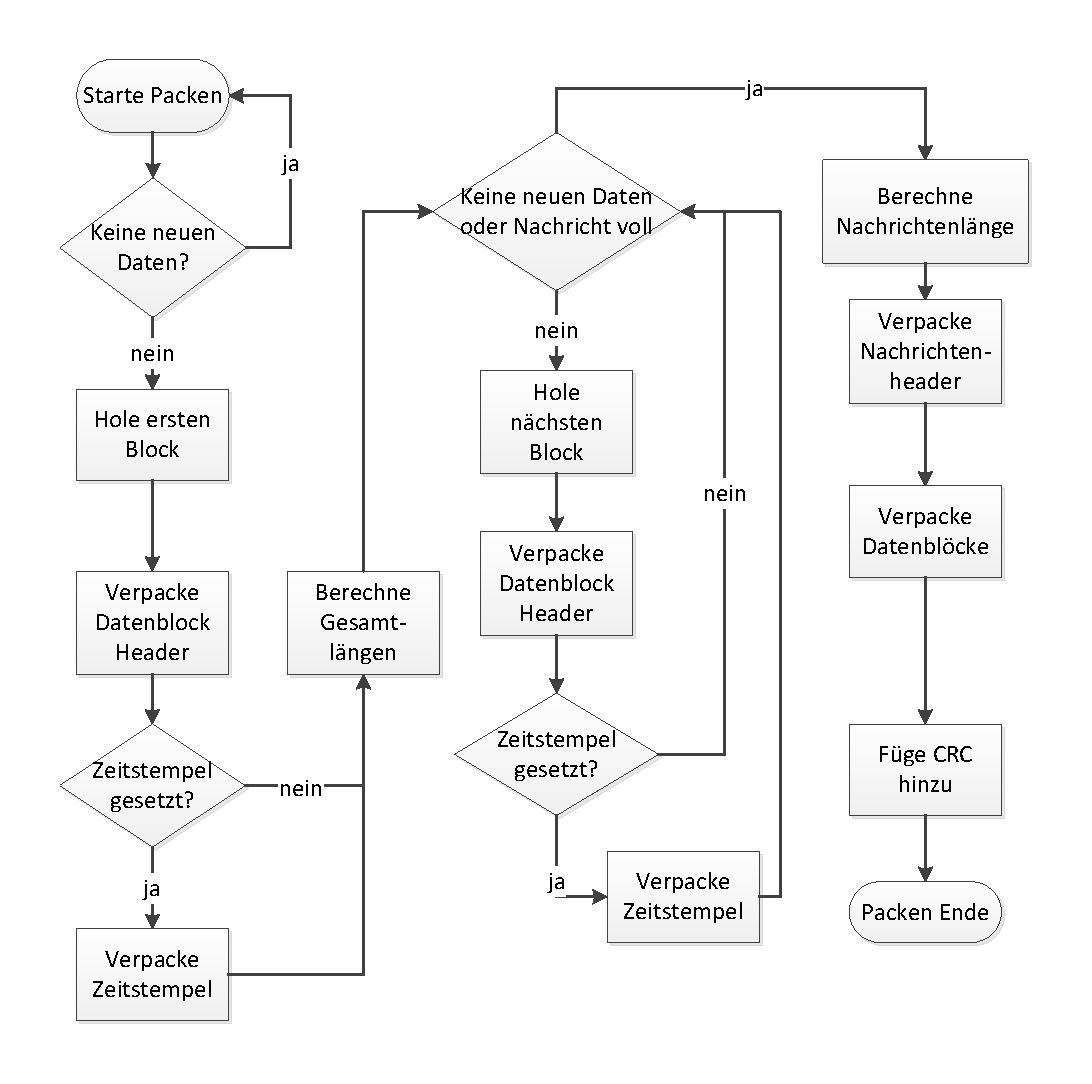
\includegraphics[scale=.5]{AlgorithmusPacketizer.pdf}
\caption{Algorithmus Packetizer}
\label{fig:AlgorithmusPacketizer}
\end{figure}

\subsection{Netzwerk}

Als Netzwerkschnittstelle wird ein UDP Socket verwendet. Dieser erh{\"a}lt die
erstellte Nachricht vom Submodul \Code{Packetizer} und leitet diese an einen
zuvor ge{\"o}ffneten UDP Socket weiter. Durch eine Client/Server basierte
Socket-Kommunikation {\"u}ber UDP (verbindungslose Kommunikation im Gegensatz
zu TCP) wird der Datenstrom an die definierte Zieladresse und den definierten
Zielport geleitet. Da es sich hierbei um eine UDP Socket-Verbindung handelt,
werden Paketverluste nicht bemerkt (keine Sicherung der Daten{\"u}bertragung).
Lediglich ein {\"u}bergreifendes Protokoll wie CROP, welches dies erkennen
k{\"o}nnte, kann dann eine erneute Sendung anfordern (zum jetzigen Zeitpunkt
ist CROP jedoch nicht f{\"a}hig einen Verbindungsabbruch zu detektieren). Die
f{\"u}r den Vorgang genutzte Adressierungsart wird im CROP Protokoll festgelegt
und somit f{\"u}r die Socket-Kommunikation {\"u}bernommen. Im Testszenario
dieser Arbeit kommt dabei IPv4 zum Einsatz.

\begin{figure}[H]
\centering
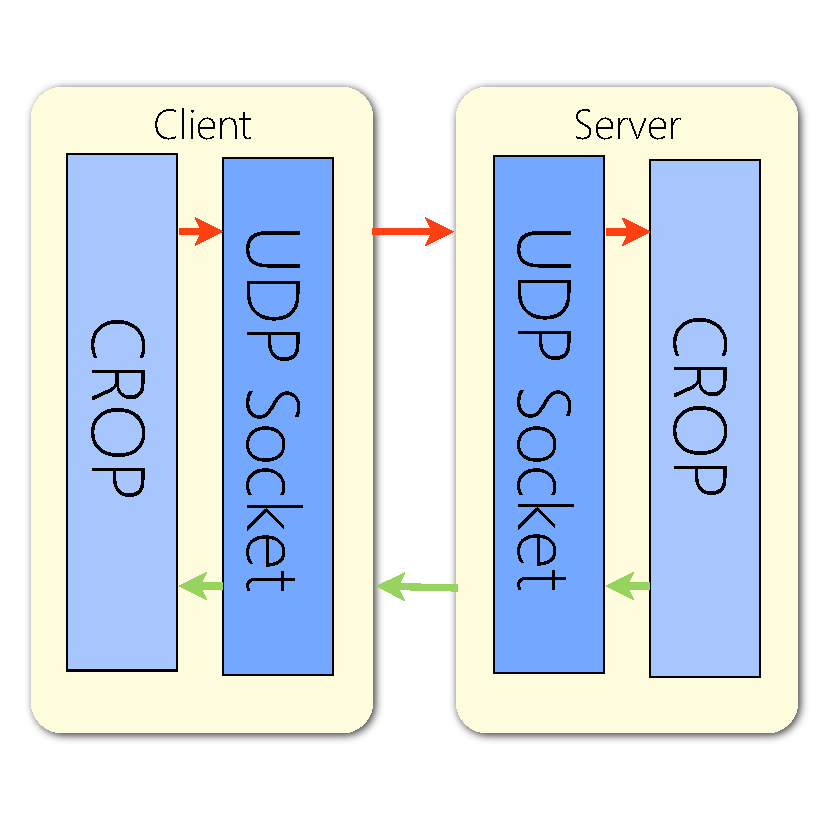
\includegraphics[scale=.5]{UDP_CROP.pdf}
\caption{Client/Server Kommunikation {\"u}ber UDP-Socket}
\label{fig:Socket-Kommunikation}
\end{figure}

Abbildung \ref{fig:Socket-Kommunikation} zeigt ein vereinfachte Dartsellung der
Socket Kommunikation zwischen Client und Server mit aufsetzendem Content
Relevance-Oriented Protocol. In Abbildung \ref{fig:OSI} erfolgt eine Einordnung
des CROP in das OSI-Referenzmodell.

\begin{figure}[H]
\centering
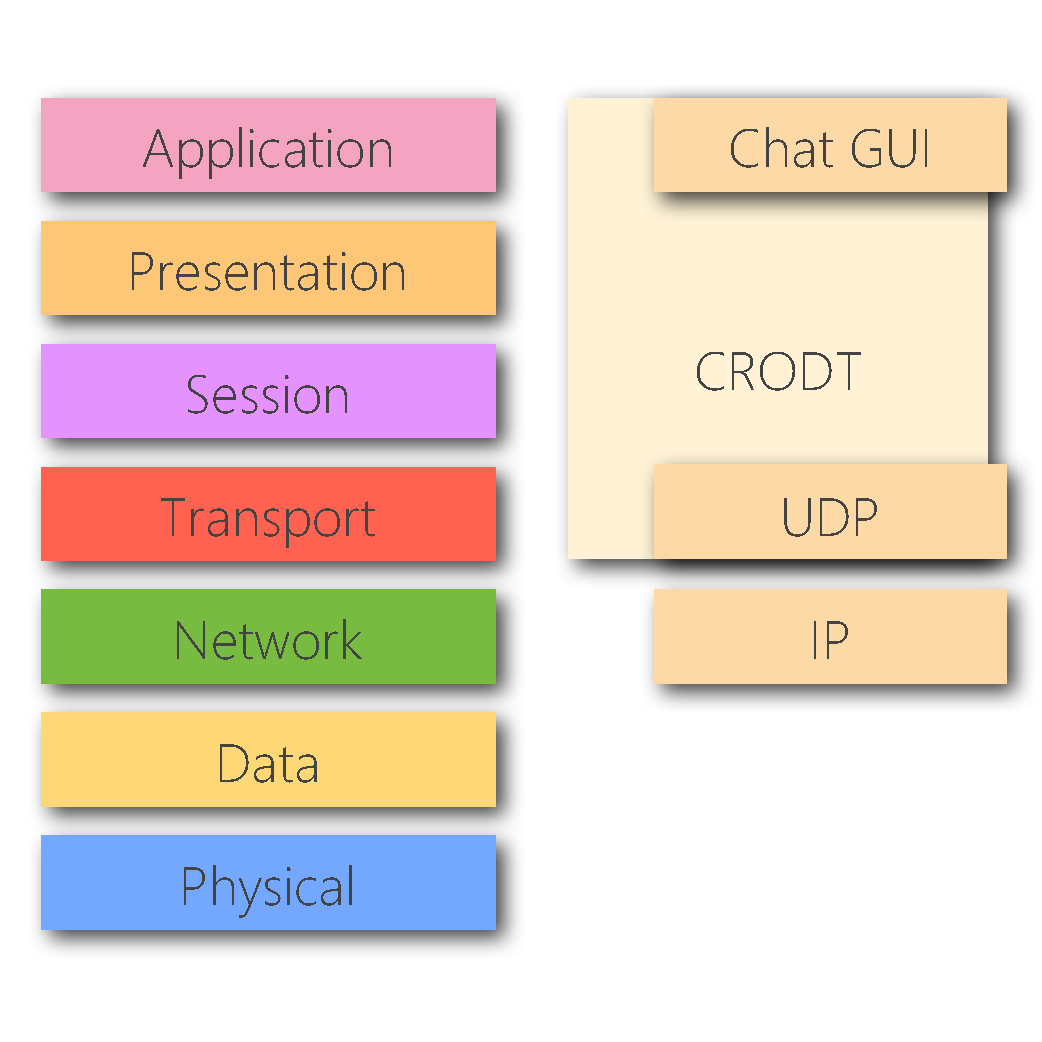
\includegraphics[scale=.38]{OSI.pdf}
\caption{{\"U}berblick des OSI-Schichtenmodells und der Zuordnung von CROP}
\label{fig:OSI}
\end{figure}



\subsection{StoreManager}

W{\"a}hrend der Entwicklung des Moduls \Code{Sender} kristallisierte sich eine
weitere notwendige Eigenschaft der Software heraus.
Die Daten, welchen w{\"a}hrend des Progammablaufes erstellt und zum Versenden
gespeichert werden, sollen auch nach einem Programmabsturz oder nach einem
Stromausfall noch vorhanden sein. Weil die Klasse \Code{SmartPrioritizedQueue}
die Daten im RAM hinterlegt, w{\"a}ren diese bei einem Absturz verloren.
F{\"u}r das Abspeichern der Daten auf die Festplatte existieren prinzipiell drei Methoden.

\begin{enumerate}
\item Jede erzeugte Variable wird direkt auf der Festplatte abgespeichert.
\item Ein Datenpaket (mehrere Variablen) wird an einer Stelle im Programm auf
einmal gespeichert.
\item Es werden Interrupts des Prozessors abgefangen, um Abst{\"u}rze zu erkennen,
infolgedessen werden alle wichtigen Daten gesichert.
\end{enumerate}

Die erste Methode hat den Vorteil, dass alle Daten sofort gesichert werden und
somit diese nicht verloren gehen k{\"o}nnen. Jedoch sind daf{\"u}r sehr viele
Festplattenzugriffe notwendig, wodurch die Laufzeit des Programms stark beeintr{\"a}chtigt wird. Bei der
dritten Methode sind die Festplattenzugriffe minimal, jedoch k{\"o}nnen nur
Software- und Hardwarefehler bei der Programmabarbeitung abgefangen werden. Bei
einem Stromausfall w{\"u}rden trotzdem alle Daten verloren gehen. Deshalb wird
Methode Zwei verwendet. Diese stellt den besten Kompromiss aus Datensicherheit
und Performance dar. \newline
F{\"u}r diese Aufgabe wurde ein Submodul entwickelt, welches die Datenbl{\"o}cke auf
der Festplatte hinterlegt und bei einem Absturz neu l{\"a}dt und damit die
\Code{SmartPrioritizedQueue} vorinitialisiert. Dadurch sind die Schnittstellen,
welche das Modul bereitstellen soll, schon indirekt vorgegeben. Diese sind, eine
Methode welche Datenbl{\"o}cke auf der Festplatte speichert, eine weitere um diese zu laden
und eine Dritte, mit der bereits gespeicherte Datenbl{\"o}cke gel{\"o}scht werden
k{\"o}nnen.

\begin{figure}[H]
\centering
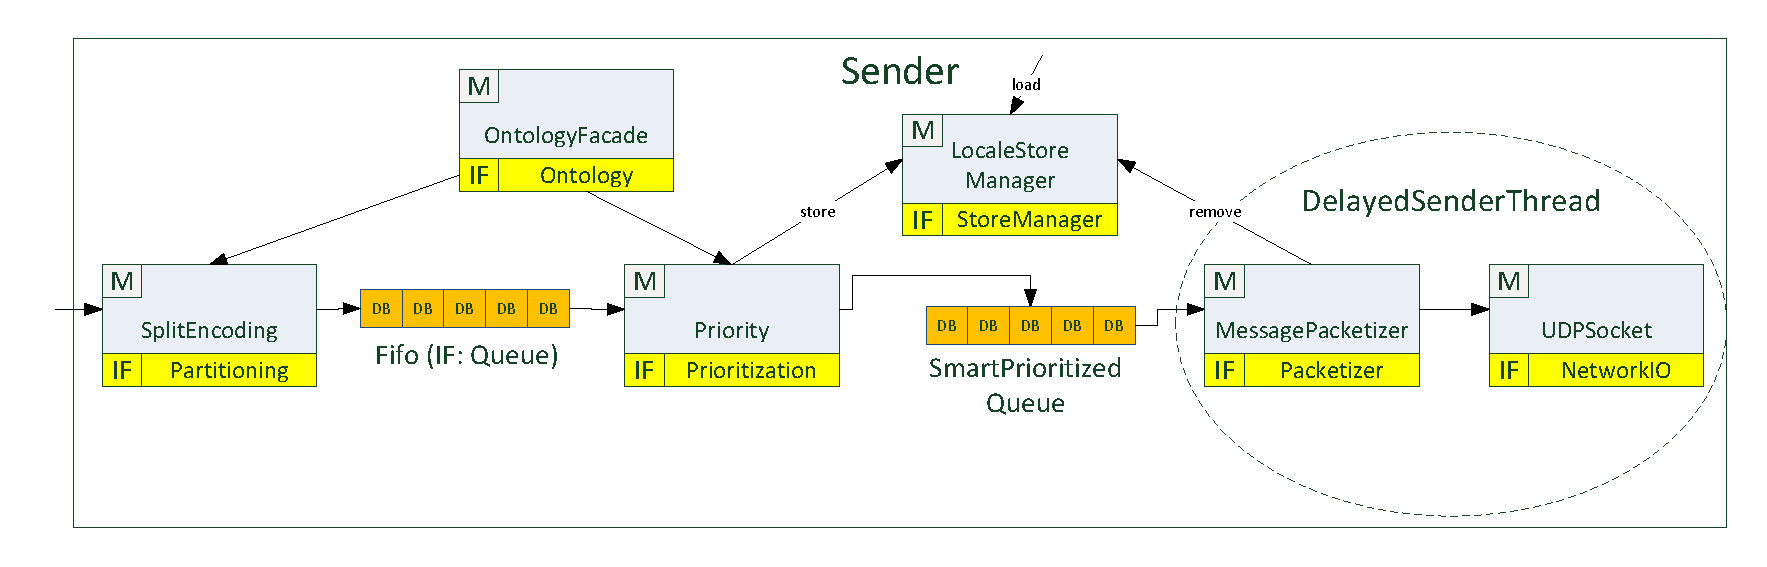
\includegraphics[scale=.5]{EinbettungStoreManager.pdf}
\caption{Integration des Submoduls \Code{StoreManager}}
\label{fig:EinbettungStoreManager}
\end{figure}

Die Einbettung des Submoduls \Code{StoreManager} in das Modul \Code{Sender} ist
in \abbildung{EinbettungStoreManager} veranschaulicht. Dazu wird der
\Code{StoreManager} parallel zur \Code{SmartPrioritizedQueue} integriert. Alle
Datenbl{\"o}cke, welche in die Queue gelangen, werden ebenfalls an die
Klasse \Code{StoreManager} {\"u}bergeben. Die von dem Submodul \Code{Packetizer}
gelesenen Datenbl{\"o}cke werden anschliesend wieder gel{\"o}scht. Somit ist immer der
aktuelle Datenbestand der \Code{SmartPrioritizedQueue}
zus{\"a}tzlich auf der Festplatte gesichert. Beim Programmstart wird in der
Initialisierungsmethode des Topmoduls {\"u}berpr{\"u}ft, ob bereits alte Daten vorhanden
sind, welche anschlie{\ss}end geladen werden. \newline
F{\"u}r das Abspeichern der
Daten fehlt noch ein passendes Dateiformat, welches ein schnelles Speichern und
Lesen erm{\"o}glicht. Dazu wurden zwei M{\"o}glichkeiten gegen{\"u}bergestellt. Diese sind
in Tabelle \ref{tab:Speicherformate} aufgef{\"u}hrt.

\begin{longtable}{|lcc|}
\caption{Vergleich der Speicherformate} \\
\hline
\label{tab:Speicherformate}
\textbf{} & \textbf{XML-Datei} & \textbf{Bin{\"a}re Datei}\\
\hline
  Menschliche Lesbarkeit      &  + & - \\
  Dateigr{\"o}{\ss}e      &  0 & + \\
  Geschwindigkeit &  0 & + \\
  Portabilit{\"a}t    &  + & - \\
\hline
\caption*{ + Gut, 0 Medium, - Schlecht }
\end{longtable}
\todo{ QUELLE???????????????????}

Der Tabelle ist zu entnehmen, dass XML auf den ersten Blick das bessere Format
ist. Dennoch wurde eine bin{\"a}re Datei verwendet, da die beiden
entscheidenden Schwachstellen (die Portabilit{\"a}t und die Lesbarkeit) f{\"u}r
einen Menschen im konkreten Anwendungsfall keine Bedeutung haben.
Weiterhin soll nur der Computer die Daten auf der Festplatte ablegen und
wieder lesen k{\"o}nnen. F{\"u}r das Versenden {\"u}ber das Internet oder
andere Medien besitzt die Portabilit{\"a}t zudem keinen gro{\ss}en Stellenwert.
Daf{\"u}r sind die beiden wichtigsten Eigenschaften, die Dateigr{\"o}{\ss}e und die
Geschwindigkeit, bei gew{\"a}hlten Format im Vergleich besser.
\newline
In der Datei werden die folgenden Daten aus dem Datenblock in der
aufgef{\"u}hrten Reihenfolge gespeichert:

\begin{itemize}
\item Datenblockheader 
\item Priorit{\"a}t
\item Zeitstempel
\item Content als ByteArray
\end{itemize}

\todo{Satz eventuell verstaendlicher formulieren ?!?}Aufgrund der Tatsache, dass
der Datenblockheader eine Kompression beinhaltet, und damit die Gr{\"o}{\ss}e der Variablen unterschiedlich sein kann, wird f{\"u}r die
Variablen festgelegt, dass f{\"u}r jeden Wert die h{\"o}chste auftretende Bitzahl
aufgerundet zur n{\"a}chsten Zweierpotenz als Byte verwendet wird. Dadurch
wird das Laden und Speichern stark vereinfacht. Der dabei auftretende zus{\"a}tzliche
Speicherplatzbedarf kann vernachl{\"a}ssigt werden.
\newline 
F{\"u}r die Ordnerstruktur wurde eine m{\"o}glichst flache Hierachie genutzt, welche in
der obersten Stufe den Ordner \Code{Backup} beinhaltet. Darin befinden sich
weitere Ordner, welche als Namen die Nummer des Datentypes beinhalten. In diesem liegen die bin{\"a}ren
Dateien deren Namen aus der Nummer der jeweiligen DOID und der
jeweiligen Sequenznummer bestehen.
Diese sind durch einen Unterstrich voneinander getrennt. Die drei Parameter
werden von der Methode remove zum L{\"o}schen einer Datei {\"u}bergeben, um diese
eindeutig zu identifizieren.

\section{Modulaufbau Empf{\"a}nger}

Auf der Empf{\"a}ngerseite sollen die ankommenden Nachrichten empfangen und geparst
werden, um an die darin enthaltenen Informationen zu gelangen. Das Empfangen
durch das Submodul \Code{UDPSocket} ist blockend. Deswegen wird der Vorgang
nebenl{\"a}ufig ausgef{\"u}hrt, damit der Programmablauf nicht behindert wird. Anschliessend wird
die Nachricht geparst und nach dem Beenden des Vorganges ein Callback
ausgel{\"o}st. Bei einem Callback wird ein Zeiger auf die Speicheradresse der
Funktion in der Klasse gespeichert. Durch Aufruf der Funktion ist es
m{\"o}glich den sequentiellen Programmablauf an einer anderen Stelle
weiterlaufen zu lassen. Nach Abarbeitung dieser kehrt der Ablauf zur
urspr{\"u}nglichen Position zur{\"u}ck. Diese Funktion kann mittels einer
Methode registriert werden, in der die geparsten Daten weiter verarbeitet werden
k{\"o}nnen.
Die Callbackfunktion k{\"o}nnte beispielsweise die Visualisierung der Daten
{\"u}bernehmen. \newline 
In \abbildung{BlockdiagrammEmpfaenger} wird eine schematische Darstellung des
Moduls angezeigt. Die Implementierung wird im Folgendem n{\"a}her erl{\"a}utert.

\begin{figure}[H]
\centering
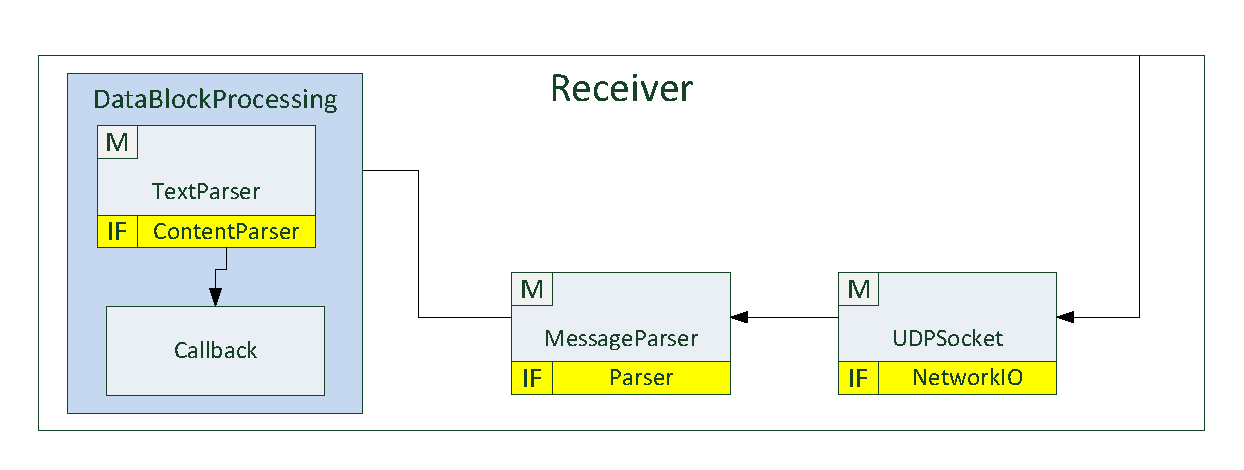
\includegraphics[scale=.5]{BlockdiagrammEmpfaenger.pdf}
\caption{{\"U}bersicht des Empf{\"a}ngers}
\label{fig:BlockdiagrammEmpfaenger}
\end{figure}

\subsection{Parser}

Der Parser basiert auf dem in Kapitel \ref{sec:ProtokolDesign}
vorgestellten Protokoll-Design.
Anhand dieser Daten wird die empfangene Nachricht Bit f{\"u}r Bit analysiert
und die Informationen herrausgezogen. 
Die Klasse \Code{UDPSocket} empf{\"a}ngt neue Daten und gibt diese an
die Klasse \Code{MessageParser} weiter. Dieser parst den Nachrichtenheader.
Dessen Algorithmus ist in \abbildung{AlgorithmusMessageParser} dargestellt.
Anschlie{\ss}end werden die Datenblockheader geparst. Der Content wird von der
Klasse \Code{DataBlockProcessing} verarbeitet.

\begin{figure}[H]
\centering
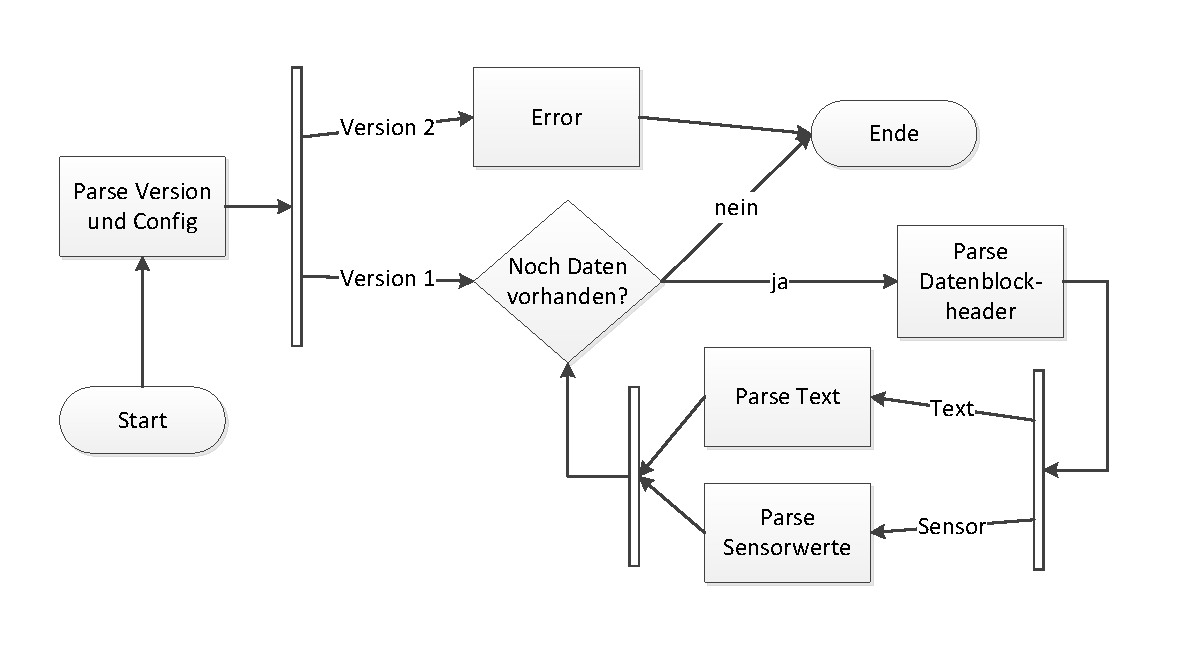
\includegraphics[scale=.5]{AlgorithmusMessageParser.pdf}
\caption{Algorithmus zum Parsen der Nachricht}
\label{fig:AlgorithmusMessageParser}
\end{figure}

Daf{\"u}r wird ein Softwarekonzept namens Policy-Based-Template-Meta Programmierung
verwendet (Ref. \cite{Alexandrescu:2001:MCD:377789}), damit die unterschiedlichen Datentypen der Datenbl{\"o}cke nach dem Parsen wieder in einem typsicheren Format vorliegen und
einfacher verwendet werden k{\"o}nnen.
Der Templateklasse werden die folgenden vier Klassen als Templateparameter
Klasse {\"u}bergeben:

\begin{itemize}
\item T - Datentyp des R{\"u}ckgabewertes des Parsers
\item Parser - Klasse zum Parsen des Datentypes
\item C - Datentyp der als Callback zur{\"u}ckgegeben wird
\end{itemize}

Der Parameter \Code{Parser} erbt zus{\"a}tzlich von einer
Schnittstelle gleichen Namens. Die Klasse \Code{DataBlockProcessing} erbt
wiederum von dem Parameter \Code{Parser}.
Dadurch besteht die M{\"o}glichkeit in der Klasse auf Funktionen und
Membervariablen zugreifen zu k{\"o}nnen.
Durch dieses Vorgehen kann das Verhalten der Klasse einfach durch die
Templateparameter ver{\"a}ndert werden. Weil der Grundalgorithmus des Parser f{\"u}r
die Datenbl{\"o}cke f{\"u}r jeden Datentyp identisch ist und lediglich die Art und
Weise ver{\"a}ndert werden muss, wie die Daten geparst werden,
ist dieser Weg der optimale. Durch das Konzept wurden
Redundanzen im Quellcode vermieden und weitere Datentypen lassen sich
sehr einfach hinzuf{\"u}gen ohne bestehenden Quellcode zu ver{\"a}ndern. Dadurch konnten
die Grundprinzipien der objektorientierten Programmierung eingehalten werden (Ref. \cite{herold2001go}).
Der eben angesprochene Grundalgorithmus, welcher f{\"u}r jeden Datentyp
durchlaufen wird, ist in Listing \ref{lst:PseudocodeDBParser} dargestellt.

\lstdefinelanguage{pseudo}{
morekeywords={if, else, for, in, remove, from, case, do, forever, to, false,
function, then, end, true, while}, sensitive=true,%
morecomment=[l]\#,%
morestring=[b]',%
}
\lstset{language=pseudo}
\lstset{commentstyle=\textit}
\lstset{literate=
 {<=} {$\le$}{2} {!=} {$\neq$}{2} {=} {$\leftarrow$}{2} {==} {=}{2} {&&}
{$\cap$}{2} {||} {$\cup$}{2} } \lstinputlisting[label=lst:PseudocodeDBParser,caption=Pseudocode
des Datenblock Parsers]
{Listings/PseudocodeDBParser.txt}
